\subsection{The CDS acceptance of the $d(K^-, n)"\pi^{\mp}\Sigma^{\pm}$}
\begin{figure}[htbp]
  \centering
  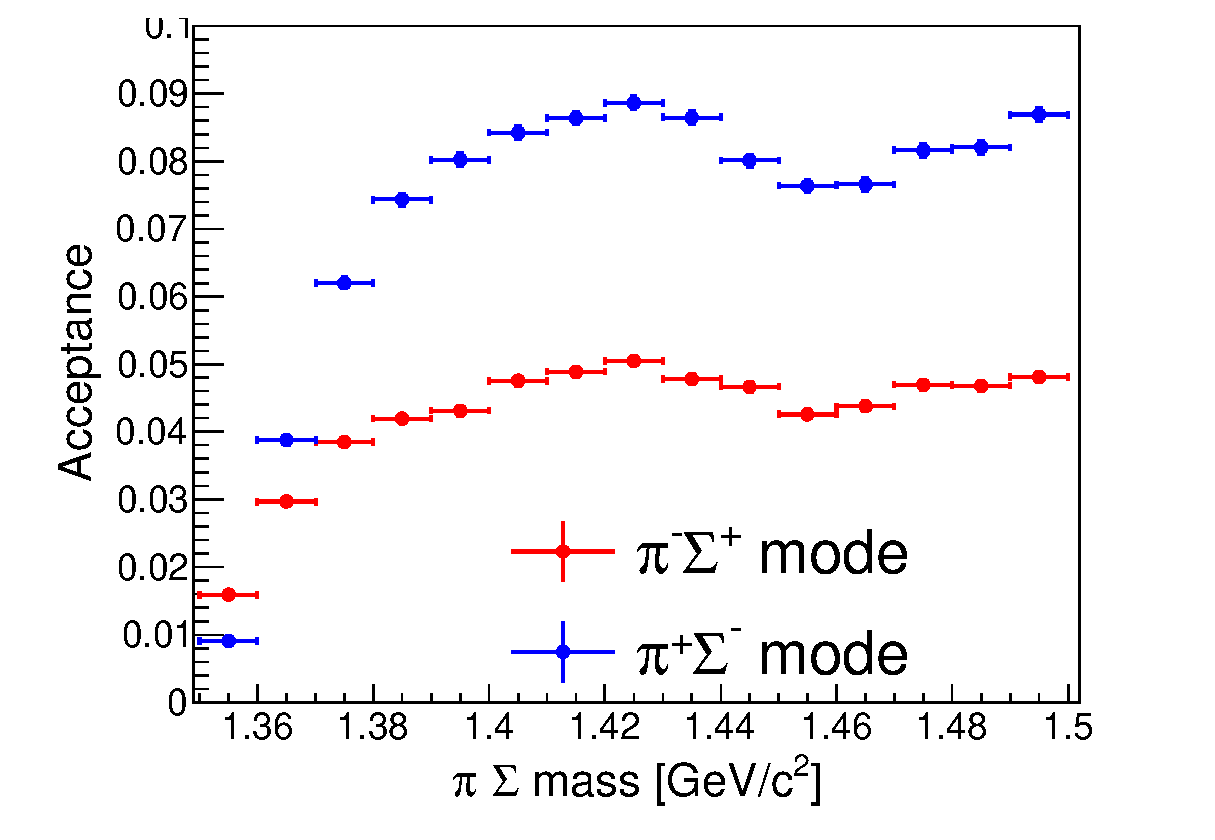
\includegraphics[width=10cm]{../pic/Run78/KN_ana_NC170_2sigma/kn_acc.eps}
  \caption{
    This figure shows the acceptance of $d(K^-, n)"\pi^{\mp}\Sigma^{\pm}"$ modes.
  }
  \label{fig:charge_mode_acc}
\end{figure}

The $d(K^-, n)"\pi^{\mp}\Sigma^{\pm}$ spectra should be collected by the CDS acceptance.
For this estimation, the $K^- d \rightarrow n_{forward} \pi^{\pm}\Sigma^{\mp}$ simulation was used.
Because the purpose of the this study is the estimated the acceptance of the CDS, the forward scattered neutron was detected event was used as the trigger events.
The same analysis procedure was adopted on the simulation data, so the acceptance was including the analysis efficiency about the CDS.
Fig\ref{fig:charge_mode_acc} indicates the acceptance of the $d(K^-, n)"\pi^{\mp}\Sigma^{\pm}$ modes.

The acceptance corrected spectra would be convered to the cross section using the luminosity and the detector efficiencies.

